\documentclass{article}
%Para imagenes
\usepackage{graphicx}
\usepackage{float}
\usepackage{enumitem} % Paquete para personalizar listas
\usepackage[margin=2cm]{geometry} % Ajusta todos los márgenes a 2 centímetros
\usepackage{indentfirst} % Este paquete fuerza la sangría del párrafo en la primera línea
\setlength{\parindent}{1cm} % Ajusta la sangría de los párrafos a 1 cm


\begin{document}
    \begin{titlepage}
        \centering
        {\bfseries\LARGE Universidad de Granada\par}
        \vspace{1cm}
        {\scshape\Large Facultad de Ingeniería Informática \par}
        \vspace{2cm}
        {\scshape\Huge Practica 2: Diseño adaptativo en Flutter \par}
        \begin{figure}[h]
                \centering
                
\includegraphics[width=0.6\textwidth]{logo_UGR.jpg}
                \label{fig:portada}
            \end{figure}
        {\itshape\Large DS: Grupo 1.7\par}
        \vfill
            {\Large  Emanuel Giraldo Herrera\par}
            {\Large  Thomas Lang \par}
            {\Large  Timur Sorokin \par}
            {\Large  Alejando Iborra Morán \par}
        \vfill
        {\Large (2023-2024) \par}
    \end{titlepage}

\tableofcontents

\newpage
\section{Abstract}

En este documento se detalla el proceso de adaptación del ejercicio 3 de la práctica 1 desarrollado en Java al nuevo framework denominado Flutter.
La tarea principal consistió en realizar el mantenimiento adaptativo y perfectivo de modo que se ha migrado de un lenguaje a otro y se añadido una interfaz gráfica para 
permitir la interacción del usuario con el sistema.

Durante el proceso de migración a Dart nos hemos encontrado con las diferencias fundamentales entre los dos lenguajes como es el caso de sintaxis y el manejo de valores NULL.

En cuanto al diseño de la interfaz de usuario (UI), se priorizó la funcionalidad sobre la estética, ya que nuestro objetivo consistia en presentar un prototipo que permitiera mostrar 
la interacción del usuario con el sistema. De modo que la interfaz se diseñó de manera sencilla y eficiente, centrándose sobretodo en la usabilidad y la claridad de la información presentada.

Finalmente, el resultado obtenido fue una pequeña aplicación que permite al usuario crear personajes seleccionando diferentes opciones y muestra los datos del personaje creado.


\section{Introducción}

En esta práctica se ha introducido un nuevo framework llamado Flutter desarrollado por Google. Este ofrece una serie de herramientas a los desarrolladores para 
crear aplicación multiplataforma con una sola base de código, es decir, el desarrollador escribe el código una vez y este puede ser compilado para diferentes plataformas como linux, windows,ios y android.

El concepto central de Flutter se basa en el uso de widgets, los cuales representan los componentes visuales de la aplicación. 
Estos widgets son altamente personalizables y pueden ser extendidos con facilidad, lo que permite a los desarrolladores crear interfaces
de usuario de manera rápida y eficiente para múltiples plataformas. Este enfoque no solo agiliza el proceso de desarrollo, sino que también 
reduce los costos asociados con el mantenimiento de aplicaciones para diferentes plataformas.

Sin embargo, a pesar de sus beneficios, Flutter también presenta algunas desventajas que deben ser consideradas:
- Curva de aprendizaje: Para los desarrolladores nuevos en Flutter, puede haber una curva de aprendizaje significativa, especialmente si no están familiarizados con el paradigma de desarrollo basado en widgets.
- Legibilidad del código con widgets anidados: En los casos donde se utilizan múltiples widgets anidados la legibilidad del código disminuy drasticamente dificultando el mantenimiento y la comprensión del código.
- Tamaño de la aplicación más grande: Debido a la inclusión del motor de Flutter y otros recursos necesarios en cada aplicación, el tamaño del ejecutable compilado suele ser más grande en comparación con las aplicaciones nativas.
- SetState repinta todos los elementos: En Flutter, el uso de la función setState() para actualizar el estado de un widget provoca que todos los elementos se vuelvan a pintar, lo que puede afectar el rendimiento de la aplicación en casos de actualizaciones frecuentes del estado.

A modo de conclusión podemos decir que a pesar de las desventajas mencionadas Flutter sigue siendo una opción relevante en el entorno de desarrollo crossplatform. Además, siendo un proyecto
respaldado por Google da cierta garantia y seguridad en cuanto al futuro de este. 

\subsection{Análisis del problema}
A partir de la información expuesta en el guion de practica se identifican claramente las siguientes dos propuestas:
- Realizar el mantenimiento adaptativo:
    Este consiste en convertir el codigo en Java obtenido en la practica anterior al Dart
- Realziar el mantenimiento perfectivo:
    Para ello introducimos una interfaz (UI) para permitir al usuario interactuar con el sistema



\subsection{Ingeniería inversa}


\newpage
\section{Desarrollo}
\subsection{Problemas encontrados}

\subsection{Widgets utilizados}

\subsection{Mejoras}



\newpage
\section{Ejecución}

\begin{figure}[h]
    \centering
    \vspace{5pt}
    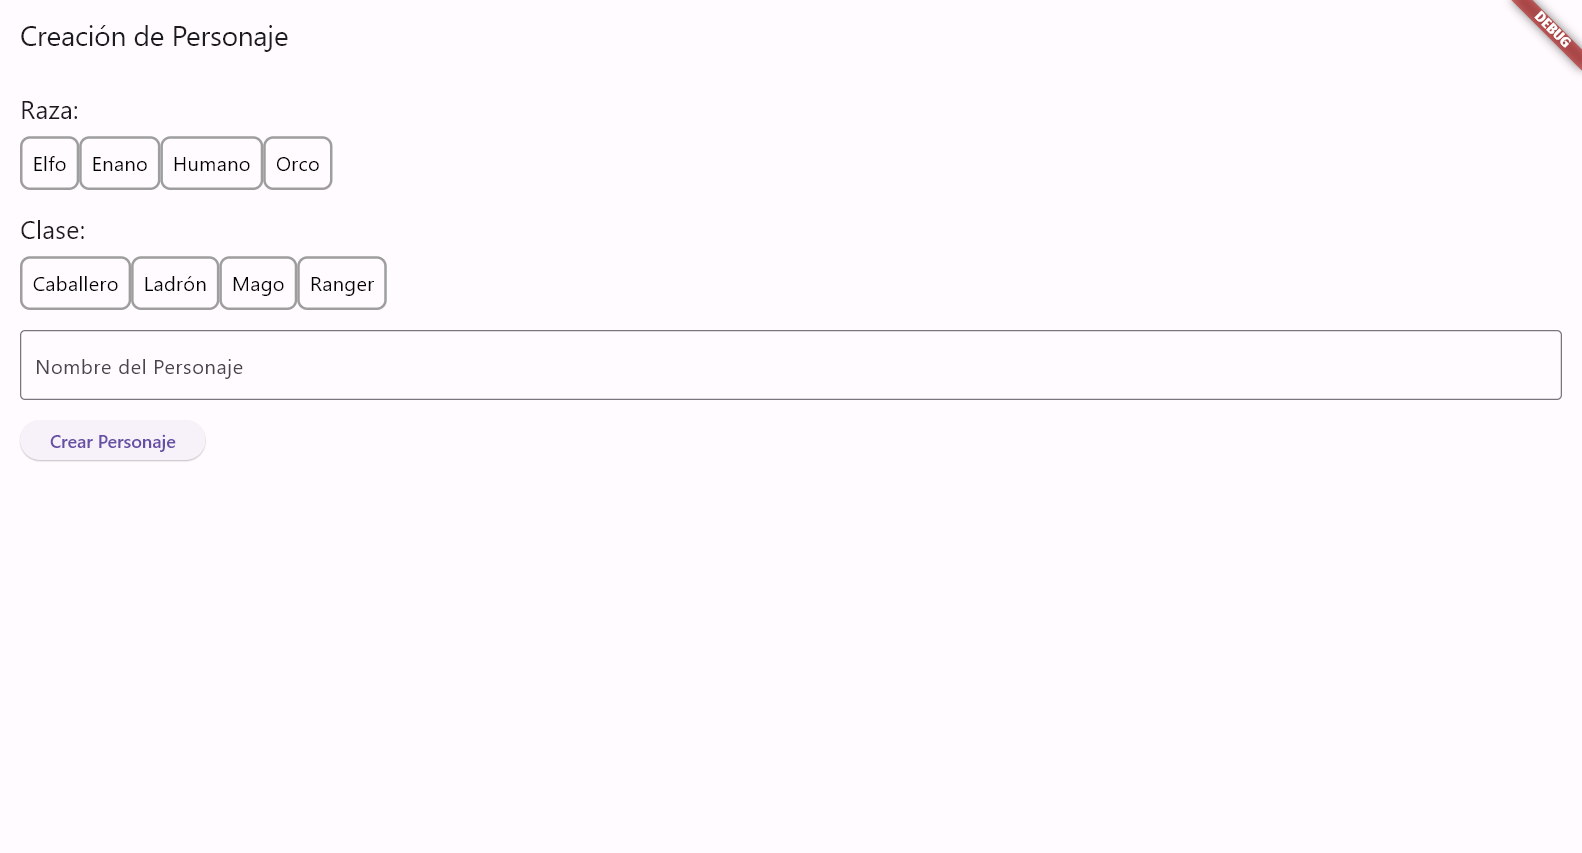
\includegraphics[width=0.9\textwidth]{Ejecucion_1.png}
    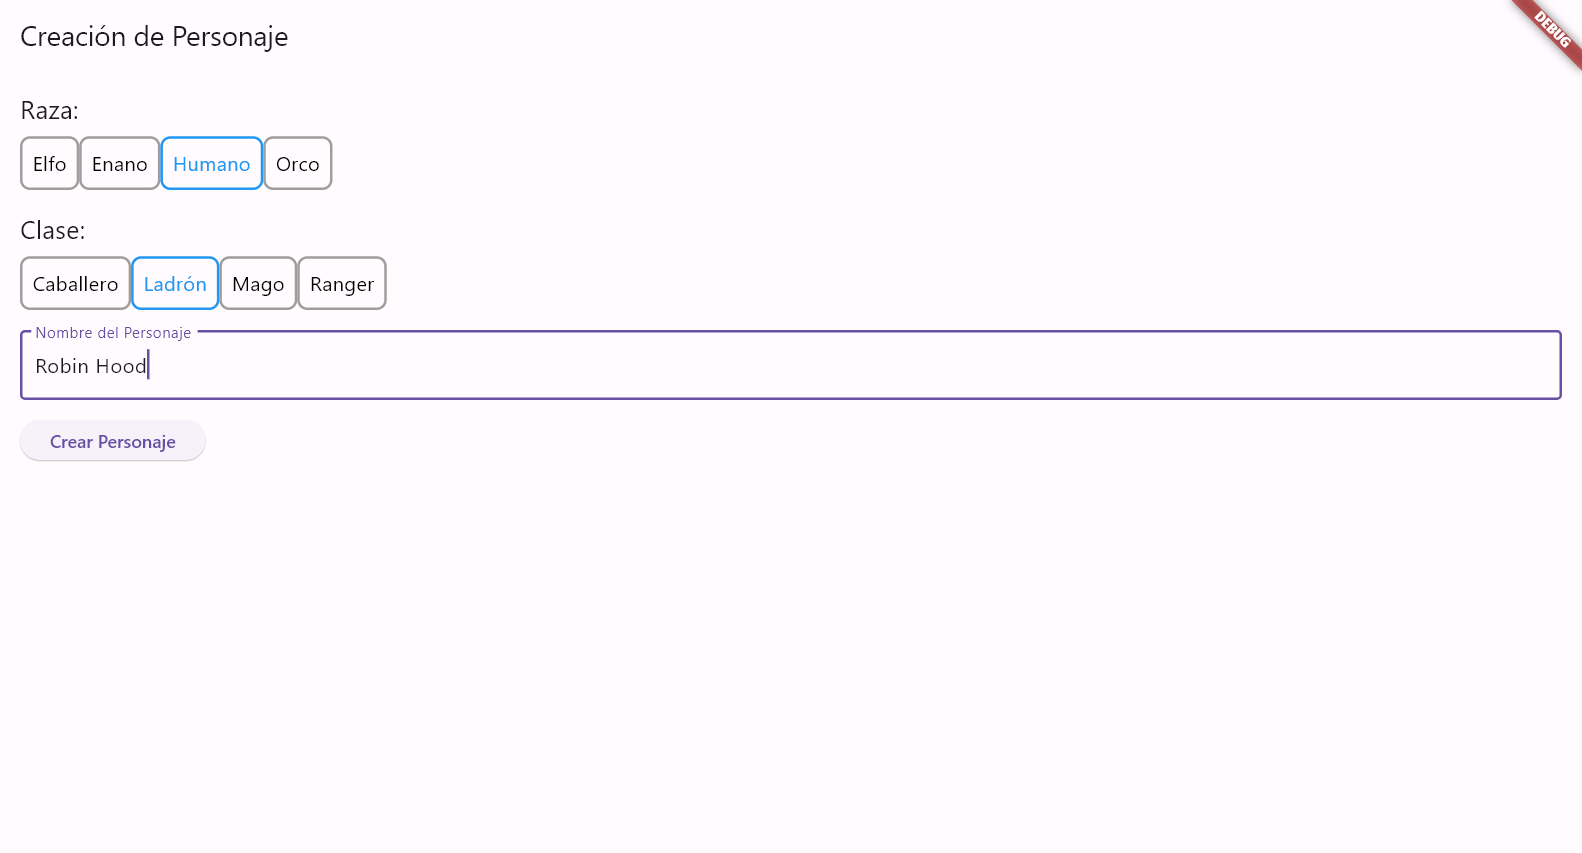
\includegraphics[width=0.9\textwidth]{Ejecucion_2.png}
    \caption{Pantalla de selección de personaje}
    \label{fig:ejecucion_1}
\end{figure}

\begin{figure}[h]
    \centering
    \vspace{5pt}
    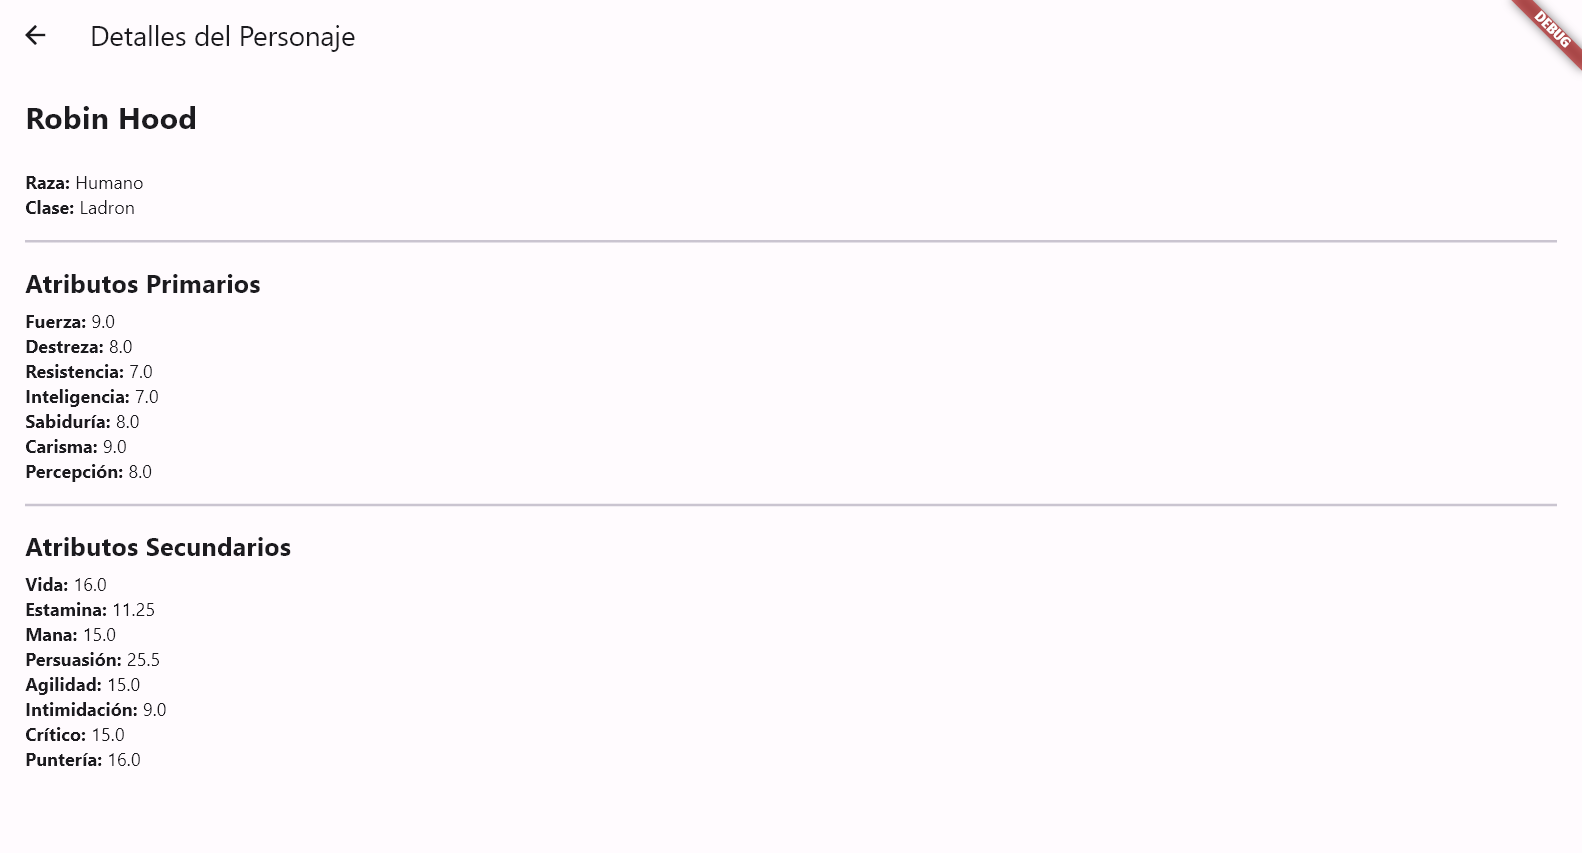
\includegraphics[width=0.9\textwidth]{Ejecucion_3.png}
    \caption{Pantalla de detalle del personaje}
    \label{fig:ejecucion_2}
\end{figure}



\end{document} 